\chapter{Sistemas da Aeronave}


\section(Sistema de Combustível)

O sistema de combustível é composto por dois tanques, um em cada asa, sendo partes constituintes da sua estrutura, conforme apresentado na \autoref{fig:sistemas_combustivel}, para o Boeing 767.

\begin{figure}
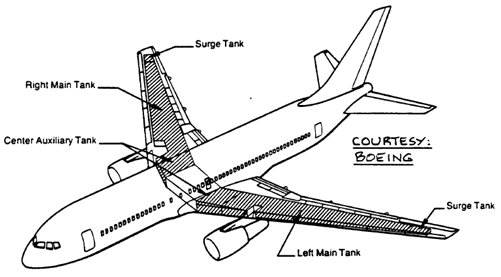
\includegraphics[width=\textwidth]{images/parte3/sistemas_combustivel.png}
\caption{Posicionamento do Sistema de Combustível}
\label{fig:sistemas_combustivel}
\end{figure}

Em condições normais, cada motor é alimentado pelo tanque da respectiva asa.
Existe, porém, uma válvula de alimentação cruzada que pode ser ativada em caso de desbalanceamento.
O volume de cada tanque é 2900 litros, e sua massa de 2250 kg.


\section{Sistema Hidráulico}

O sistema hidráulico é dividido em dois, sendo, cada um, pressurizado por uma bomba eletrica.
O primeiro sistema é responsável por alimentar os flaps, os spoilers, o movimento do trem de pouso de nariz, os freios das hélices, os freios de emergência e os freios de estacionamento.
Já o segundo sistema alimenta o acionamento dos trens de pouso (incluindo a frenagem normal dos trens de pouso principais).
A pressão de operação é de 3000 PSI.
Assim como no caso do sistema de combustível, existe uma válvula de alimentação cruzada que possibilita a troca entre as bombas no caso de falha de alguma delas.
O sistema é representado na \autoref{fig:sistemas_hidraulico}:

\begin{figure}
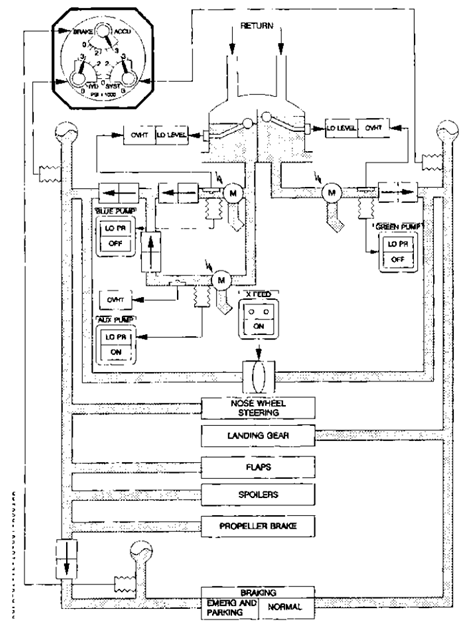
\includegraphics[width=\textwidth]{images/parte3/sistemas_hidraulico.png}
\caption{Representação esquemática do Sistema Hidráulico}
\label{fig:sistemas_hidraulico}
\end{figure}


\section{Trem de pouso}

O trem de pouso é do tipo triciclo, sendo recolhido na fuselagem, conforme definido na primeira parte do projeto.
A \autoref{fig:sistemas_trem_de_pouso} representa o funcionamento do trem de pouso principal.

\begin{figure}
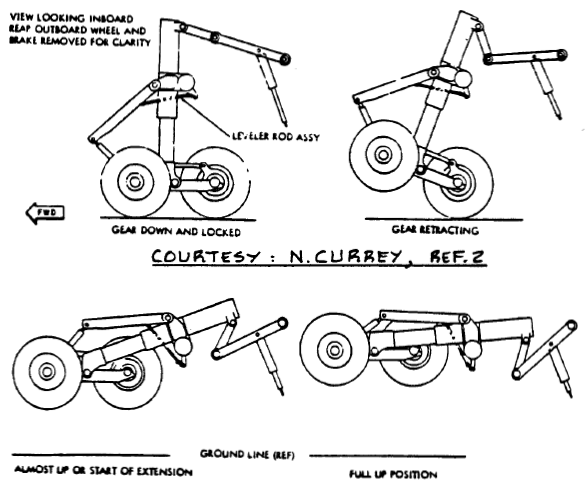
\includegraphics[width=\textwidth]{images/parte3/sistemas_trem_de_pouso.png}
\caption{Representação da operação de recolhimento do trem de pouso principal}
\label{fig:sistemas_trem_de_pouso}
\end{figure}


\section{Sistemas Auxiliares do motor}

\subsection{Sistema de Injeção de Água}

Para garantir que a redução da densidade do ar em dias quentes não acarrete uma grande perda de potência no motor, é necessário que haja um sistema de refrigeração dos motores, que neste caso consistirá na injeção de agua misturada com metanol diretamente na câmara de combustão, permitindo assim uma recuperação de até 100\% na potência de decolagem.

A injeção do liquido refrigerante é feita através de uma bomba acionada pneumaticamente pelo ar sob alta pressão proveniente do compressor.
A injeção causa um aumento de fluxo dos gases na turbina e uma redução da sua temperatura, o que permite, respectivamente, um aumento na pressão do tubo de descarga e na RPM, que, por sua vez, causam um aumento na tração.

\subsection{Sistema de Lubrificação}

É necessário lubrificar os rolamentos e o conjunto de engrenagens do motor, o que é feito com óleo lubrificante, o qual também tem como função refrigerar os rolamentos e realizar a variação do passo e embandeiramento da hélice.
O sistema consiste em um ciclo fechado, onde o óleo, após realizar suas funções, retorna ao reservatório.

\subsection{Sistema de Partida e Ignição}

O sistema de partida é do tipo pneumático, sendo interrompido quando a rotação do conjunto compressor-turbina atinge um valor de 60\% da velocidade normal de operação.
A escolha deste sistema se deve a sua leveza, simplicidade e economia, além de ser possível iniciar sua operação a partir da APU da aeronave.

O sistema de ignição é responsável principalmente por reacender o motor em altitudes elevadas, onde a baixa temperatura causa um decréscimo na volatilidade do combustível.
Ele tem por objetivo produzir centelhas que queimarão a mistura ar/combustivel.

\subsection{Sistema de Proteção e Extinção de Incêndio}

Por motivos de segurança, todas as tubulações de fluidos inflamáveis são isoladas da região quente do motor, sendo os tubos de combustível fabricados em material resistente a fogo.
Além disso, há um sistema dedicado à detecção de fogo, constituído de um termocouple que é ativado na presença de fogo e envia um sinal eletrico para o alarme, que, por sua vez, só é desarmado quando o detector esfria, ou seja, após o fogo ser apagado.
Já o sistema de extinção é conforme a \autoref{fig:sistemas_extincao_incendio}, para uma aeronave turbo-fan.

\begin{figure}
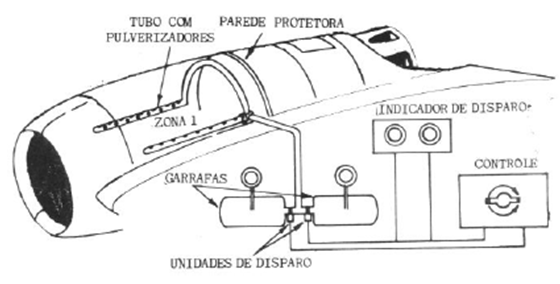
\includegraphics[width=\textwidth]{images/parte3/sistemas_extincao_incendio.png}
\caption{Representação esquemática do Sistema de Extinção de Incêndio, para uma aeronave turbo-fan}
\label{fig:sistemas_extincao_incendio}
\end{figure}


\section{Sistema de Ambientação}

\subsection{Sistema de Ar Condicionado}

Para garantir o conforto térmico dos passageiros e tripulantes, o sistema de ar condicionado deve ser capaz de manter a temperatura dentro da cabine entre 18°C e 26°C.

O FAR-25 estabelece mais alguns requisitos de conforto, a saber: ventilação de 0,5 Lb/min em condições normais de operação e sistema de alarme que impossibilite a penetração de fumaça na cabine.

O sistema de ar-condicionado é do tipo ciclo a ar e consiste de duas unidades de controle ambiental (packs) localizados acima do compartimento do trem de pouso principal, que atuam de forma automática e independente, conforme ilustrado na \autoref{fig:sistemas_ambientacao}, para um Boeing 767.

\begin{figure}
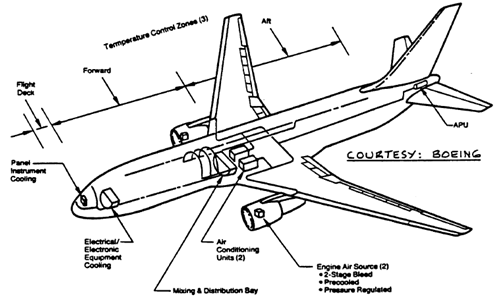
\includegraphics[width=\textwidth]{images/parte3/sistemas_ambientacao.png}
\caption{Posicionamento das unidade de controle ambiental (packs) do Sistema de Ar Condicionado}
\label{fig:sistemas_ambientacao}
\end{figure}

Seu funcionamento inicia a partir da admissão de ar quente sangrado do motor, que é comprimido e resfriado nos packs, sendo então misturado ao ar proveniente da ventilação da cabine.
Após esse processo, o ar é então redirecionado à cabine.
A \autoref{fig:sistemas_ambientacao_esquema} ilustra o funcionamento.

\begin{figure}
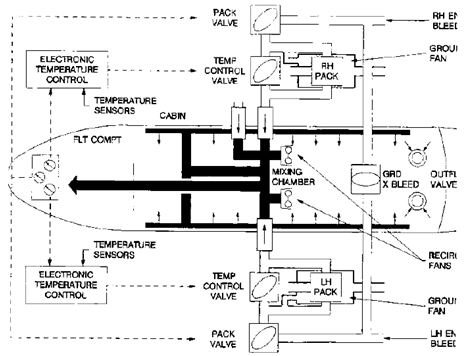
\includegraphics[width=\textwidth]{images/parte3/sistemas_ambientacao_esquema.png}
\caption{Representação esquemática do Sistema de Ar Condicionado}
\label{fig:sistemas_ambientacao_esquema}
\end{figure}

É importante notar que a ventilação da cabine conta com um sistema de admissão do ar exterior, e também de remoção do ar interno para o ambiente, o que permite um maior controle dos contaminantes em suspenção (como vírus, por exemplo).
A \autoref{fig:sistemas_ambientacao_esquema_2} mostra como ocorre a ventilação dentro da cabine.

\begin{figure}
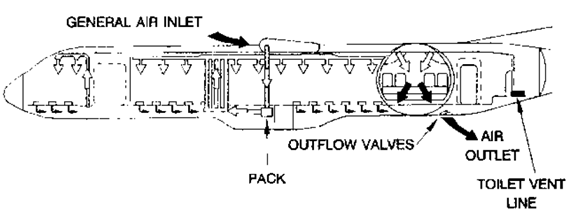
\includegraphics[width=\textwidth]{images/parte3/sistemas_ambientacao_esquema_2.png}
\caption{Esquema de ventilação da cabine}
\label{fig:sistemas_ambientacao_esquema_2}
\end{figure}

\subsection{Sistema de Pressurização}

O sistema de pressurização é responsável por manter a pressão interna a níveis toleráveis para os tripulantes da aeronave nos voos a altas altitudes.
Esse controle é realizado por um sistema totalmente automatizado, que mede a pressão externa e atua motores elétricos para comprimir o ar interno, impedindo a sobre pressão através do acionamento de válvulas outflow.
A \autoref{fig:sistemas_pressurizacao} representa esse processo.

\begin{figure}
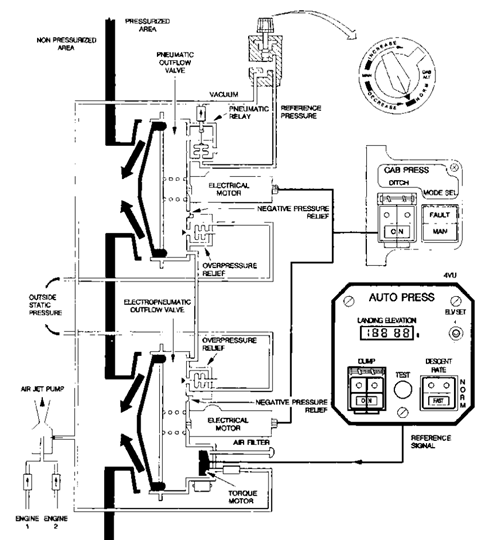
\includegraphics[width=\textwidth]{images/parte3/sistemas_pressurizacao.png}
\caption{Representação esquemática do Sistema de Pressurização}
\label{fig:sistemas_pressurizacao}
\end{figure}


\section{Sistema de Antigelo e Degelo}

Este sistema tem por objetivo impedir a formação e gelo e suas consequências, dentre as quais: perca de eficiência aerodinâmica das superfícies sustentadoras devido a deformação geométrica, erros de medição dos tubos de Pitot e falta de visibilidade para o piloto.

Seu funcionamento se dá pela utilização de dois sistemas: um sistema pneumático acionado pelo ar sangrado do motor que atua nas superfícies aerodinâmicas e outro de aquecimento eletrico, que atua nos tubos de Pitot, para-brisas e pás da hélice.
A \autoref{fig:sistemas_antigelo_degelo} mostra o princípio de funcionamento.

\begin{figure}
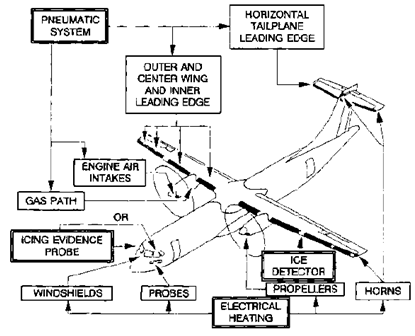
\includegraphics[width=\textwidth]{images/parte3/sistemas_antigelo_degelo.png}
\caption{Representação esquemática do Sistema de Antigelo e Degelo}
\label{fig:sistemas_antigelo_degelo}
\end{figure}


\section{Sistema Elétrico}

O sistema eletrico é provido por duas baterias e uma APU (Auxiliary Power Unit), localizada na cauda da aeronave, conforme ilustrado na \autoref{fig:sistemas_eletrico}, de um MacDouglas.

\begin{figure}
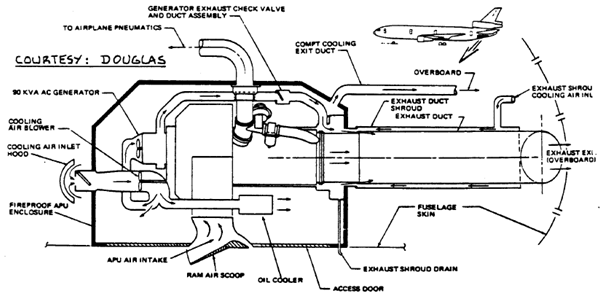
\includegraphics[width=\textwidth]{images/parte3/sistemas_eletrico.png}
\caption{Representação esquemática da APU}
\label{fig:sistemas_eletrico}
\end{figure}

\section{Sistemas de Instrumentação, Navegação e Comunicação}

Esses sistemas consistem de toda a aviônica presente na aeronave, e também de outros equipamentos, como antenas e luzes.
A aviônica não será discutida em detalhes, visto que é a última parte a ser integrada na aeronave.
Na \autoref{fig:sistemas_instrumentacao} é representada a localização das antenas.

\begin{figure}
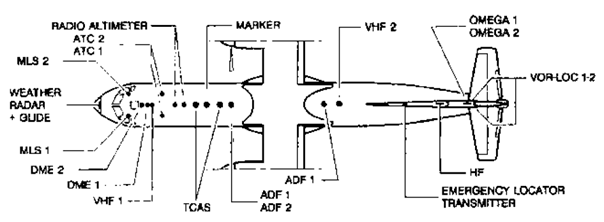
\includegraphics[width=\textwidth]{images/parte3/sistemas_instrumentacao.png}
\caption{Posicionamento das antenas}
\label{fig:sistemas_instrumentacao}
\end{figure}
